\documentclass[lualatex,aspectratio=169]{beamer}
\usepackage[T1]{fontenc}
\usepackage{luatexja}
\usepackage{luatexja-ruby}
\usepackage[deluxe]{luatexja-preset}
\usepackage{amsmath}
\usepackage{tikz}
\usetikzlibrary{shapes.geometric, positioning, arrows.meta, calc}
\usepackage{caption}
\captionsetup[figure]{labelformat=empty}
\setmainjfont{Hiragino Kaku Gothic ProN}

\usetheme[progressbar=none]{metropolis}

\usepackage{pifont}
\newcommand{\cmark}{\ding{51}}%
\newcommand{\xmark}{\ding{55}}%


\usepackage{xcolor}
\definecolor{hf-orange}{HTML}{FFA700}
\definecolor{hf-orange-dark}{HTML}{FF882B}
\definecolor{hf-blue}{HTML}{4884DA}
\definecolor{hf-blue-dark}{HTML}{4D6BD5}
\definecolor{hf-orange-gradient-left}{HTML}{FF882B}
\definecolor{hf-orange-gradient-right}{HTML}{FFE721}
\definecolor{hf-blue-gradient-left}{HTML}{48D2E6}
\definecolor{hf-blue-gradient-right}{HTML}{4D6BD5}
\definecolor{white}{HTML}{FFFFFF}

\setbeamertemplate{footline}{%
  \begin{tikzpicture}[remember picture, overlay]
    % left half of the bar
    \shade[left color=hf-orange-gradient-left, right color=hf-orange-gradient-right]
      (current page.south west) rectangle ([yshift=0.5mm]current page.south);

    % right half of the bar
    \shade[left color=hf-blue-gradient-left, right color=hf-blue-gradient-right]
      (current page.south) rectangle ([yshift=0.5mm]current page.south east);

    % slide number
    \node[
      anchor=east,
      xshift=-5mm,
      yshift=5mm,
      font=\sffamily\color{mDarkTeal}
    ]
    at (current page.south east)
    {\insertframenumber};
  \end{tikzpicture}%
}

\setbeamertemplate{title separator}{
  
\begin{tikzpicture}
    % Left half of the bar
    \shade[left color=hf-orange-gradient-left, right color=hf-orange-gradient-right]
      (0,0) rectangle (0.5\textwidth, 0.25mm);
    % Right half of the bar
    \shade[left color=hf-blue-gradient-left, right color=hf-blue-gradient-right]
      (0.5\textwidth,0) rectangle (\textwidth, 0.25mm);
  \end{tikzpicture}
  \vskip1em % Adds a little vertical space after the separator
}

\setbeamertemplate{section page}{
  \begin{center}
    \usebeamerfont{section title}
    \usebeamercolor[fg]{section title}
    \insertsection
    \par % Creates a new paragraph for spacing
    
\begin{tikzpicture}
      % Left half of the bar
      \shade[left color=hf-orange-gradient-left, right color=hf-orange-gradient-right]
        (0,0) rectangle (0.5\textwidth, 0.25mm);
      % Right half of the bar
      \shade[left color=hf-blue-gradient-left, right color=hf-blue-gradient-right]
        (0.5\textwidth,0) rectangle (\textwidth, 0.25mm);
    \end{tikzpicture}
  \end{center}
}

\setbeamercolor{frametitle}{fg=mDarkTeal, bg=black!2}
\setbeamertemplate{frametitle}{
  \nointerlineskip%
  \begin{tikzpicture}
    % use the full paper width and a height of 5ex
    \useasboundingbox (0,0) rectangle (\paperwidth, 5ex);

    % background for the entire header
    \fill[black!2] (0,0) rectangle (\paperwidth, 5ex);

    % thin gradient bar on the left (top to bottom)
    \shade[top color=hf-orange-gradient-left, bottom color=hf-orange-gradient-right] (0,0) rectangle (1.5mm, 5ex);

    % frame title text (mDarkTeal on black!2)
    \node[
      anchor=west,      % align text to the left
      inner xsep=1em,     % add padding between bar and text
      text=mDarkTeal
    ] at (2mm, 2.5ex) { % position the node
      \usebeamerfont{frametitle}\insertframetitle
    };
  \end{tikzpicture}%
}

% --- helpers --------------------------------------------------------------

% show TikZ elements only on certain overlays: [visible on=<2->]
\tikzset{
  invisible/.style={opacity=0, text opacity=0},
  visible on/.style={alt={#1{}{invisible}}},
  alt/.code args={<#1>#2#3}{\alt<#1>{\pgfkeysalso{#2}}{\pgfkeysalso{#3}}},
}

% mock-up of an Anki card on a phone
% #1: card content, #2: buttons at the bottom
% \phonecard puts the content at the top, \phonecardcenter in the middle
\newcommand{\phoneframe}[2]{%
  \begin{tikzpicture}[x=1cm, y=1cm]
    \draw[rounded corners=4mm, line width=1.2pt, fill=white] (0,0) rectangle (3.2,6.0);
    \fill[black!80, rounded corners=0.5mm] (1.25,5.70) rectangle (1.95,5.78);
    \draw[black!20] (0.15,0.35) rectangle (3.05,5.55);
    #1
    \node[anchor=south, text width=2.8cm, align=center] at (1.6,0.5) {#2};
  \end{tikzpicture}%
}
\newcommand{\phonecard}[2]{\phoneframe{%
  \node[anchor=north, text width=2.8cm, align=center] at (1.6,5.25) {#1};}{#2}}
\newcommand{\phonecardcenter}[2]{\phoneframe{%
  \node[anchor=center, text width=2.8cm, align=center] at (1.6,3.1) {#1};}{#2}}

% keep the compound in one piece when lines wrap
\newcommand{\kotei}{\mbox{高低アクセント}}

% first column width shared by the two small tables in the self-intro
\newlength{\introcol}

% data as it appears in a file (file name tab, box with content)
% #1: file name, #2: content
\newcommand{\datafile}[2]{%
  \begin{tikzpicture}
    \node[anchor=north west, fill=black!80, text=white, inner sep=3pt,
          font=\ttfamily\tiny, rounded corners=1pt] (tab) at (0,0) {#1};
    \node[anchor=north west, fill=black!5, draw=black!20, inner xsep=6pt, inner ysep=5pt,
          font=\ttfamily\small] (line) at (tab.south west) {#2};
  \end{tikzpicture}%
}
% the 図書館 entry of the Wadoku XML dump as CSV, header named after the
% XML elements (orth, hira, hatsuon, accent); #1: the accent field
% columns are padded after the commas so the fields line up
\newcommand{\toshokancsv}[1]{%
  \begin{tabular}{@{}r@{\hspace{1em}}l@{\hspace{.5em}}l@{\hspace{.5em}}l@{\hspace{.5em}}l@{}}
    {\color{black!35}1} & {\color{black!55}orth,} & {\color{black!55}hira,}
      & {\color{black!55}hatsuon,} & {\color{black!55}accent}\\
    {\color{black!35}2} & 図書館, & としょかん, & としょ･かん, & #1
  \end{tabular}}
\newcommand{\toshokandata}[1]{\datafile{wadoku.csv}{\toshokancsv{#1}}}

% top-aligned code in a fixed-size box, small enough that no line wraps
\newcommand*{\csscode}[1]{\parbox[t][1.6cm][t]{3.1cm}{%
  \ttfamily\fontsize{4.6pt}{5.8pt}\selectfont #1}}

\setbeamerfont{title}{size=\LARGE}
\setbeamerfont{subtitle}{size=\footnotesize}
\setbeamercolor{subtitle}{fg=black!55}
\newcommand{\cardbutton}[2]{{\setlength{\fboxsep}{2pt}\colorbox{#1}{\strut #2}}}
\newcommand{\frontbuttons}{{\scriptsize\cardbutton{black!10}{答えを表示}}}
\newcommand{\backbuttons}{{\fontsize{4.5pt}{5pt}\selectfont%
  \cardbutton{red!15}{もう一度}\hspace{1pt}%
  \cardbutton{orange!20}{難しい}\hspace{1pt}%
  \cardbutton{green!15}{正解}\hspace{1pt}%
  \cardbutton{blue!12}{簡単}}}
\newcommand{\cardfront}{{\large library}}
\newcommand{\cardsep}{\\[2pt]{\color{black!25}\rule{2.4cm}{0.4pt}}\\[6pt]}
\newcommand{\cardback}{\cardfront\cardsep{\LARGE 図書館}\\[4pt]{\small としょかん}}
\newcommand{\cardbackpitch}{\cardfront\cardsep{\LARGE 図書館}\\[4pt]%
  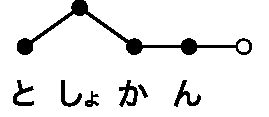
\includegraphics[width=2.2cm]{./img/toshokan_mora.pdf}}

% recreation of the overline notation (high morae overlined, drop marked)
\newcommand{\overlinenotation}{%
  \begin{tikzpicture}[baseline=(t.base)]
    \node[inner sep=0] (t) {ト};
    \node[inner sep=0, anchor=west] (s) at (t.east) {ショ};
    \node[inner sep=0, anchor=west] (k) at (s.east) {カン};
    \draw[line width=1.5pt]
      ([yshift=3pt]s.north west) -- ([yshift=3pt]s.north east)
      -- ([yshift=-6pt]s.north east);
  \end{tikzpicture}%
}

% --- content --------------------------------------------------------------

\title{欲しいものはオープンに作る}
\subtitle{暗記カードアプリに高低アクセントを自動で付けるアドオン}
\author{tarek（タレク）}
\date{東海道らぐ ライトニングトーク大会 @ KOF 2026}

\begin{document}

\begin{frame}[plain]
  \titlepage
\end{frame}

\begin{frame}[t]{自己紹介}
    \begin{itemize}
        \item tarek（タレク）\onslide<2->{\hphantom{mmmmm}エンジニア@ \raisebox{-0.13cm}{
\includegraphics[height=0.5cm]{./img/helpfeel_logo.pdf}}}
        \onslide<3->{\item 日本との関わり\\[.3em]
        {\small\settowidth{\introcol}{2024年6月〜}%
        \hspace*{1.2em}\begin{tabular}{@{}p{\introcol}l}
            2013年 & 日本語の勉強を始める\\
            2015年 & 交換留学で1年間日本へ\\
            2024年6月〜 & 日本在住（大阪）
        \end{tabular}}}
        \onslide<4->{\item 趣味\\[.3em]
        {\small\settowidth{\introcol}{2024年6月〜}%
        \hspace*{1.2em}\begin{tabular}{@{}p{\introcol}l}
            個人開発 & \\
            Linux & 2010年〜（現在はDebian）
        \end{tabular}}}
    \end{itemize}
\end{frame}

\begin{frame}[t]{背景}
    \begin{columns}[T,onlytextwidth]
    \begin{column}{0.64\textwidth}
        \vskip1.5em
        \textbf{Anki}
        \begin{itemize}
            \item OSSの暗記カードアプリ
            \item 語学に限らず、何でもカードにできる
            \item ユーザーが作ったデッキが多数公開されている
        \end{itemize}
    \end{column}
    \begin{column}{0.32\textwidth}
        \begin{center}
        \only<1>{\phonecardcenter{\cardfront}{\frontbuttons}}%
        \only<2>{\phonecard{\cardback}{\backbuttons}}%
        \end{center}
    \end{column}
    \end{columns}
\end{frame}

\begin{frame}[t]{動機}
    \begin{columns}[T,onlytextwidth]
    \begin{column}{0.55\textwidth}
        \vskip.5em
        \begin{itemize}
            \item 自分の単語カード（5,000枚以上）に\kotei{}を付けたい
            \onslide<2->{\item 既存のアドオンの表記はしっくりこない}
            \onslide<3->{\item 欲しかったのは『大辞林』のような図}
            \onslide<4->{\item[$\rightarrow$] 自分で作ることに}
        \end{itemize}
    \end{column}
    \begin{column}{0.4\textwidth}
        \vskip1.5em
        \begin{center}
        \onslide<2->{{\Huge\overlinenotation}}\\[2.5em]
        \onslide<3->{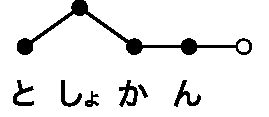
\includegraphics[width=.75\linewidth]{./img/toshokan_mora.pdf}}
        \end{center}
    \end{column}
    \end{columns}
\end{frame}

\begin{frame}[t]{作ったもの}
    \begin{columns}[T,onlytextwidth]
    \begin{column}{0.6\textwidth}
        \vskip1.5em
        \begin{tikzpicture}[
            box/.style={draw=mDarkTeal, rounded corners=2pt, align=left, inner sep=5pt, font=\small},
            arr/.style={-{Stealth[length=2mm]}, line width=0.8pt, mDarkTeal},
            lbl/.style={font=\scriptsize, text=mDarkTeal},
          ]
          \node[box] (in) at (0,0) {表記：図書館\\読み：としょかん};
          \node[draw=mDarkTeal, cylinder, shape border rotate=90, aspect=0.25,
                minimum width=1.8cm, minimum height=1.3cm, font=\small,
                visible on=<2->] (db) at (4.4,0) {データ};
          \node[visible on=<3->] (svg) at (4.4,-2.4)
                {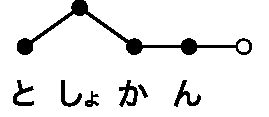
\includegraphics[width=2.2cm]{./img/toshokan_mora.pdf}};
          \draw[arr, visible on=<2->] (in) -- node[lbl, above] {検索} (db);
          \draw[arr, visible on=<3->] (db) -- node[lbl, right] {SVGを生成} (svg);
          \draw[arr, visible on=<4->] (svg.east) -- ++(1.6,0) node[lbl, above, pos=0.5] {カードへ};
        \end{tikzpicture}
        \vskip1em
        \onslide<5->{{\footnotesize 画像ファイル不要・CSSで見た目を調整可能}}
    \end{column}
    \begin{column}{0.36\textwidth}
        \begin{center}
        \only<1-3>{\phonecard{\cardback}{\backbuttons}}%
        \only<4->{\phonecard{\cardbackpitch}{\backbuttons}}%
        \end{center}
    \end{column}
    \end{columns}
\end{frame}

\begin{frame}[t]{オープンデータ}
    \begin{itemize}
        \item 必要なもの：機械可読で、再配布できる\kotei{}のデータ
        \onslide<2->{\item[$\rightarrow$] Wadoku（和独辞典）：有志による和独辞書プロジェクト}
    \end{itemize}
    \vskip.2em
    {\centering
    \onslide<2->{%
        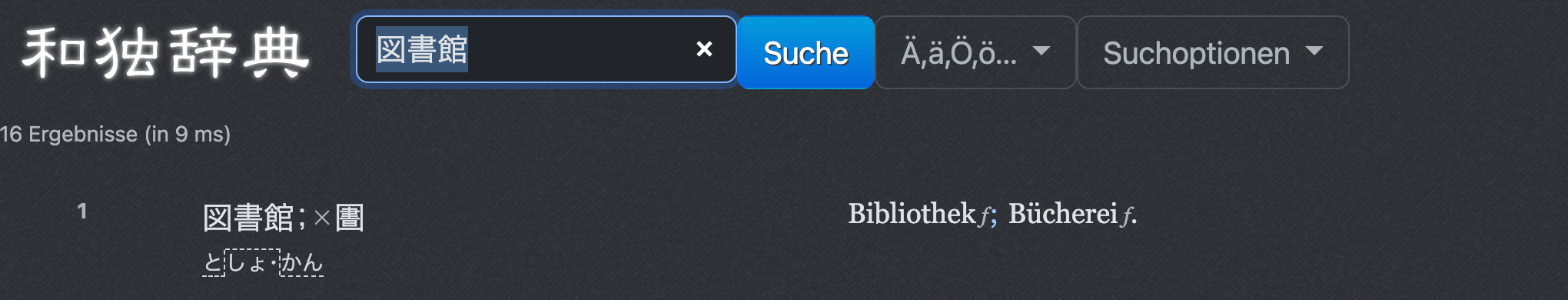
\includegraphics[width=.66\linewidth]{./img/wadoku_toshokan.png}\\[-.2em]
        {\fontsize{4pt}{5pt}\selectfont\texttt{wadoku.de}}\par}
    \vskip.3em
    \onslide<3->{%
        \toshokandata{2}\par}
    }
    \onslide<4->{
        \vskip.5em
        {\scriptsize Wadoku.de-Daten Lizenz 5.3：無料で配布するソフトウェアへの組み込みが可能（データの出典を明記）\par}
        {\fontsize{4.5pt}{5pt}\selectfont\texttt{\url{https://wadoku.de/wiki/display/WAD/Wadoku.de-Daten+Lizenz}}\par}
    }
\end{frame}

\begin{frame}[t]{作って学んだこと}
    \begin{center}
    \toshokandata{{\setlength{\fboxsep}{1pt}\colorbox{hf-orange!40}{2}}}
    % question only before the illustrations appear (frees up space below)
    \only<1>{\\[.3em]{\scriptsize 「2」＝ 2番目の後で下がる……何の2番目？}}
    \end{center}
    \vskip-.2em
    \begin{columns}[T,onlytextwidth]
    \begin{column}{0.48\textwidth}
        \onslide<2->{{\centering
        文字で数える\\[.4em]
        \begin{tabular}{ccccc}
            と & \colorbox{hf-orange!40}{し} & ょ & か & ん\\
            \scriptsize 1 & \scriptsize\textbf{2} & \scriptsize 3 & \scriptsize 4 & \scriptsize 5
        \end{tabular}\\[.6em]
        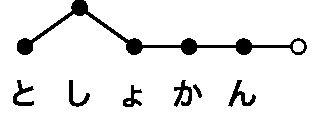
\includegraphics[width=.6\linewidth]{./img/toshokan_char.pdf}\\
        {\Large\color{red!70!black}\xmark}\par}
        }
    \end{column}
    \begin{column}{0.48\textwidth}
        \onslide<3->{{\centering
        モーラで数える\\[.4em]
        \begin{tabular}{cccc}
            と & \colorbox{hf-orange!40}{しょ} & か & ん\\
            \scriptsize 1 & \scriptsize\textbf{2} & \scriptsize 3 & \scriptsize 4
        \end{tabular}\\[.6em]
        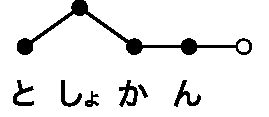
\includegraphics[width=.5\linewidth]{./img/toshokan_mora.pdf}\\
        {\Large\color{green!50!black}\cmark}\par}
        }
    \end{column}
    \end{columns}
\end{frame}

\begin{frame}[t]{コントリビューター}
    \begin{itemize}
        \item アドオンのユーザーがIssue・PRを作ってくれる
    \end{itemize}
    \vskip.8em
    % numbers last, but placed above the timeline (\onslide keeps their space)
    \onslide<5->{
    \begin{columns}[T,onlytextwidth]
    \begin{column}{0.32\textwidth}
        \begin{center}
        {\Huge 48,448}\\[.2em]
        {\small ダウンロード}
        \end{center}
    \end{column}
    \begin{column}{0.32\textwidth}
        \begin{center}
        {\Huge 47}\\[.2em]
        {\small 人がIssue・PRを作成}
        \end{center}
    \end{column}
    \begin{column}{0.32\textwidth}
        \begin{center}
        {\Huge 3}\\[.2em]
        {\small 人がコードで貢献}
        \end{center}
    \end{column}
    \end{columns}
    }
    \vskip1.5em
    % timeline first: full axis, milestones revealed one by one
    \begin{center}
    \begin{tikzpicture}[x=1.35cm, font=\scriptsize]
        % x = years since 2019-01-01; ticks/labels mark the start of each year
        \draw[line width=1pt, mDarkTeal] (0,0) -- (8,0);
        \foreach \y [count=\i from 0] in {2019,...,2026} {
            \draw[mDarkTeal] (\i,-0.08) -- (\i,0.08);
            \node[below=2pt, text=black!60] at (\i,0) {\y};
        }
        % milestones at their actual dates (fraction of the year);
        % labels on two levels so neighbouring ones don't overlap
        %   2019-09-01  release on AnkiWeb
        %   2020-05-12  first issue by someone else (#2)
        %   2022-01-23  first outside code merged (PR #23)
        %   2026-10-07  most recent outside code merged (PR #68)
        \foreach \x/\lvl/\txt/\ov in {0.67/0.35/公開/1, 1.36/0.8/最初のIssue/2, 3.06/0.35/外部コード初マージ/3, 7.77/0.35/直近のコントリビューター/4} {
            \begin{scope}[visible on=<\ov->]
                \draw[black!30] (\x,0) -- (\x,\lvl);
                \fill[hf-orange] (\x,0) circle (3pt);
                \node[above=1pt, text=black] at (\x,\lvl) {\txt};
            \end{scope}
        }
    \end{tikzpicture}
    \end{center}
    \vfill
    \onslide<5->{{\tiny ダウンロード数：AnkiWeb（2026年11月時点）、その他：GitHub}}
\end{frame}

\begin{frame}[t]{方針とユーザーの要望}
    \begin{columns}[T,onlytextwidth]
    \begin{column}{0.58\textwidth}
        \vskip.5em
        方針
        \begin{itemize}
            \item 外部ライブラリに依存しない
            \item ユーザーのデータはなるべく触らない
        \end{itemize}
        \onslide<2->{
        \vskip.6em
        要望の例
        \begin{itemize}
            \item ダークモード用CSSの自動追加のPR
            \begin{itemize}
                \item ユーザーのCSSを解析・書き換え
                \item[$\rightarrow$] 議論してクローズ
            \end{itemize}
        \end{itemize}
        }
    \end{column}
    \begin{column}{0.38\textwidth}
        \vskip3.5em
        \begin{center}
        % night mode: the user's own card styling the PR would have edited
        \onslide<2->{
            {\tiny ユーザーのカードのCSS}\\[.2em]
            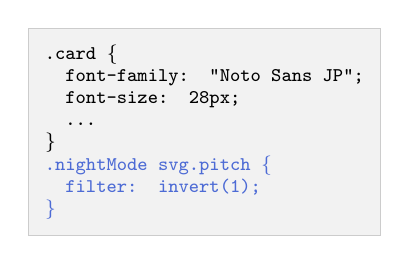
\begin{tikzpicture}
                \node[fill=black!5, draw=black!20, align=left, inner sep=6pt,
                      font=\ttfamily\scriptsize] {%
                    .card \{\\
                    \hspace{1em}font-family: "Noto Sans JP";\\
                    \hspace{1em}font-size: 28px;\\
                    \hspace{1em}...\\
                    \}\\
                    \textcolor{hf-blue-dark}{.nightMode svg.pitch \{}\\
                    \hspace{1em}\textcolor{hf-blue-dark}{filter: invert(1);}\\
                    \textcolor{hf-blue-dark}{\}}};
            \end{tikzpicture}
        }
        \end{center}
    \end{column}
    \end{columns}
\end{frame}

% gag: many ways to write night mode CSS (the PR's line-based check would
% only find the first one; variants taken from the review on PR #67)
\begin{frame}[t]{余談：ダークモードのCSS、何通り？}
    \centering
    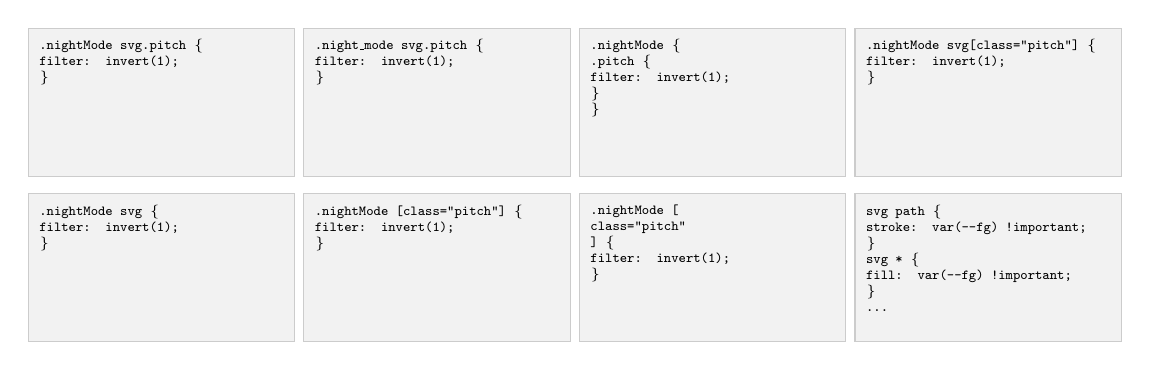
\begin{tikzpicture}[
        css/.style={fill=black!5, draw=black!20, inner sep=4pt, anchor=north west},
      ]
      % x/y positions of the 2x4 grid
      \def\gx{3.5} \def\gy{2.1}
      \node[css] at (0,0) {\csscode{%
        .nightMode svg.pitch \{\\
        \ \ filter: invert(1);\\
        \}}};
      \node[css] at (\gx,0) {\csscode{%
        .night\_mode svg.pitch \{\\
        \ \ filter: invert(1);\\
        \}}};
      \node[css] at (2*\gx,0) {\csscode{%
        .nightMode \{\\
        \ \ .pitch \{\\
        \ \ \ \ filter: invert(1);\\
        \ \ \}\\
        \}}};
      \node[css] at (3*\gx,0) {\csscode{%
        .nightMode svg[class="pitch"] \{\\
        \ \ filter: invert(1);\\
        \}}};
      \node[css] at (0,-\gy) {\csscode{%
        .nightMode svg \{\\
        \ \ filter: invert(1);\\
        \}}};
      \node[css] at (\gx,-\gy) {\csscode{%
        .nightMode [class="pitch"] \{\\
        \ \ filter: invert(1);\\
        \}}};
      \node[css] at (2*\gx,-\gy) {\csscode{%
        .nightMode [\\
        \ \ class="pitch"\\
        ] \{\\
        \ \ filter: invert(1);\\
        \}}};
      \node[css] at (3*\gx,-\gy) {\csscode{%
        svg path \{\\
        \ \ stroke: var(-{}-fg) !important;\\
        \}\\
        svg * \{\\
        \ \ fill: var(-{}-fg) !important;\\
        \}\\
        ...}};
    \end{tikzpicture}
    \par\vfill
    {\scriptsize PRでの議論：\texttt{\url{https://github.com/IllDepence/anki_add_pitch_plugin/pull/67}}}
\end{frame}

\begin{frame}[t]{まとめ}
    \begin{center}
    {\Large 欲しいものはオープンに作る}
    \end{center}
    \vskip.5em
    \begin{itemize}
        \onslide<2->{\item Wadoku：有志がオープンに作ってくれた辞書データ
        \begin{itemize}
            \item[$\rightarrow$] おかげでアドオンが作れた
        \end{itemize}}
        \onslide<3->{\item アドオン：自分が欲しかったツールをオープンに
        \begin{itemize}
            \item[$\rightarrow$] 他の人の「欲しい」にもなり、改善も集まる
        \end{itemize}}
    \end{itemize}
\end{frame}

\begin{frame}[t]{ご清聴ありがとうございました}
    tarek（タレク）
    \begin{columns}
    \begin{column}{0.3\textwidth}
        \begin{center}
        \begin{figure}
        
\includegraphics[width=0.7\textwidth]{./img/qr_github.png}
        \end{figure}
        \footnotesize GitHub
        \end{center}
    \end{column}
    \begin{column}{0.3\textwidth}
        \begin{center}
        \begin{figure}
        
\includegraphics[width=0.7\textwidth]{./img/qr_ankiweb.png}
        \end{figure}
        \footnotesize AnkiWeb
        \end{center}
    \end{column}
    \begin{column}{0.3\textwidth}
        \begin{center}
        \begin{figure}
        
\includegraphics[width=0.7\textwidth]{./img/qr_slides.png}
        \end{figure}
        \footnotesize スライド
        \end{center}
    \end{column}
    \end{columns}
\end{frame}

\end{document}
